%% 
%% Copyright 2007-2020 Elsevier Ltd
%% 
%% This file is part of the 'Elsarticle Bundle'.
%% ---------------------------------------------
%% 
%% It may be distributed under the conditions of the LaTeX Project Public
%% License, either version 1.2 of this license or (at your option) any
%% later version.  The latest version of this license is in
%%    http://www.latex-project.org/lppl.txt
%% and version 1.2 or later is part of all distributions of LaTeX
%% version 1999/12/01 or later.
%% 
%% The list of all files belonging to the 'Elsarticle Bundle' is
%% given in the file `manifest.txt'.
%% 

%% Template article for Elsevier's document class `elsarticle'
%% with numbered style bibliographic references
%% SP 2008/03/01
%%
%% 
%%
%% $Id: elsarticle-template-num.tex 190 2020-11-23 11:12:32Z rishi $
%%
%%
\documentclass[preprint,12pt]{elsarticle}

%% Use the option review to obtain double line spacing
%% \documentclass[authoryear,preprint,review,12pt]{elsarticle}

%% Use the options 1p,twocolumn; 3p; 3p,twocolumn; 5p; or 5p,twocolumn
%% for a journal layout:
%% \documentclass[final,1p,times]{elsarticle}
%% \documentclass[final,1p,times,twocolumn]{elsarticle}
%% \documentclass[final,3p,times]{elsarticle}
%% \documentclass[final,3p,times,twocolumn]{elsarticle}
%% \documentclass[final,5p,times]{elsarticle}
%% \documentclass[final,5p,times,twocolumn]{elsarticle}

%% For including figures, graphicx.sty has been loaded in
%% elsarticle.cls. If you prefer to use the old commands
%% please give \usepackage{epsfig}

%% The amssymb package provides various useful mathematical symbols
\usepackage{booktabs}
\usepackage{amssymb}
\usepackage{graphicx}
\usepackage{amsmath}
%\usepackage{mathtools}
%% The amsthm package provides extended theorem environments
%% \usepackage{amsthm}

%% The lineno packages adds line numbers. Start line numbering with
%% \begin{linenumbers}, end it with \end{linenumbers}. Or switch it on
%% for the whole article with \linenumbers.
%% \usepackage{lineno}

\journal{Optik}

\begin{document}

\begin{frontmatter}

%% Title, authors and addresses

%% use the tnoteref command within \title for footnotes;
%% use the tnotetext command for theassociated footnote;
%% use the fnref command within \author or \address for footnotes;
%% use the fntext command for theassociated footnote;
%% use the corref command within \author for corresponding author footnotes;
%% use the cortext command for theassociated footnote;
%% use the ead command for the email address,
%% and the form \ead[url] for the home page:
%% \title{Title\tnoteref{label1}}
%% \tnotetext[label1]{}
%% \author{Name\corref{cor1}\fnref{label2}}
%% \ead{email address}
%% \ead[url]{home page}
%% \fntext[label2]{}
%% \cortext[cor1]{}
%% \affiliation{organization={},
%%             addressline={},
%%             city={},
%%             postcode={},
%%             state={},
%%             country={}}
%% \fntext[label3]{}

\title{Theoretical study to optimize the yield of $InGaN/Si$ tandem solar cell using Solcore.}

%% use optional labels to link authors explicitly to addresses:
%%\author[label1,label3]{}
%% \affiliation[label1]{organization={},
%%             addressline={},
%%             city={},
%%             postcode={},
%%             state={},
%%             country={}}
%%
%% \affiliation[label2]{organization={},
%%             addressline={},
%%             city={},
%%             postcode={},
%%             state={},
%%             country={}}

\author{Abdelwahab Douha\fnref{label1}}
\ead{doha@gmail.com}
\affiliation[label1]{organization={University Tahri Mohamed of Bechar},
            addressline={B.P 417 route kenadsa}, 
            postcode={08.000}, 
            state={Bechar},
            country={Algeria}}
\author{Benameur Amiri\corref{cor1}\fnref{label2}}            
%\author{Benameur Amiri\fnref{label2}}
\ead{lpdsamis@gmail.com}
%% \ead[url]{home page}
%%\fntext[label2]{}
\cortext[cor1]{Benameur Amiri}
\affiliation[label2]{organization={Higher Normal School of Bechar},
				 addressline={B.P. 601, Route de Kenadsa},
	             postcode={08.000},
	             state={Bechar},
	             country={Algeria}}
\author{Abdelrahmane Belghachi\fnref{label1}}
\ead{abelghachi@yahoo.fr}

\begin{abstract}
Optical and electrical properties of $InGaN$ alloys is being intensively studied to be combined with silicon by implementing $SiO_{2}/Si3N4$ interlayers. Adhesion of nano-interlayer appears to reduce photonic electro-migration hurdle between $InGaN$ and $Si$, in order to achieve high-efficiency solar cell. However, a relatively thick layer of $InGaN$ is difficult to grow due to the relaxation issue in material. This issue can be avoided by eboxy layer. This work, we present an $InGaN/Si$ tandem solar cell modeled using Wien2k and Solcore softwares. We have shown that 25\% of indium is needed to ensure the current matching between the top cell and the bottom cell. With feasible structural parameters, we have shown that an efficiency near to 30\% can be achieved with $InGaN/Si$ tandem cell.
\end{abstract}

\begin{keyword}
%% keywords here, in the form: keyword 
Solcore \sep Wien2k code \sep III-Ns \sep Tandem solar cell \sep eboxy layer.
%% PACS codes here, in the form: \PACS code \sep code

%% MSC codes here, in the form: \MSC code \sep code
%% or \MSC[2008] code \sep code (2000 is the default)
\end{keyword}
\end{frontmatter}
%% \linenumbers
%% main text
\section{Introduction} \label{sec:Int}
III-nitride $(N)$ semiconductors, including aluminum nitride $(AlN)$, gallium nitride $(GaN)$, and indium nitride $(InN)$, are highly promising building for optoelectronics and high-power electronics \cite{strite1992gan}. the III-nitrides have wurtzite crystal structure at ambient conditions, and the direct band-gap changes from 6.2 eV of $AlN$, 3.4 eV of $GaN$, to 0.7 eV of $InN$. III-Ns are displaying large amount of commercialized optoelectronics devices, including Photodetectors \cite{pernot2000solar,chen1997schottky,munoz1997photoconductor}, light-emitting diodes (LEDs) (\cite{nakamura1993high,funato2006blue,iso2007high}, laser diodes (LDs) \cite{nakamura1998continuous}, and solar cells \cite{neufeld2008high,jani2007design,jiang2017enhanced},which are applied in energy harvesting. Compared to other semiconductors, III-Ns demonstrate a fundamental advantage of the formation of heterogeneous structures, such as quantum wells, and  quantum dots. Heterogeneous structures $III-N$ can be manufactured through key crystal growth techniques, including molecular beam epitaxy (MBE), metal-organic chemical vapor deposition (MOCVD) and hydride vapor-phase epitaxy (HVPE) \cite{jain2000iii,yoshida1982properties,li2007influence}.Due to the inability of a single solar cell to absorb large solar spectrum photons efficiently, multijunction solar cells have been the focus of much theoretical and experimental work in the past few decades. The most successful efforts to date have focused on the use of semiconductors such as II-VI and III-V alloys to construct such cells, achieving energy conversion efficiencies of over 30\%. The $InGaN$ range band gap can be engineered from 0.7 to 3.4 eV, and this makes it suitable for a range of multijunction solar cell designs. These cells are able to use high-energy photons more efficiently than those limited to band gaps of less than 1.8 eV. These cells will also have the advantage that $Si$ is relatively cheap and abundant as well as that the $Si$ range gap of 1.2 eV is ideally suited to the lower connection of a high-efficiency two-link solar cell. Growth of $InGaN$-based opto-electronic device structures on $Si$ has been extensively investigated previously with the goal of optimizing the interface layers between the $Si$ and the active layers to reduce defects in the nitride layers and to improve device performance. Hsu et al.\cite{hsu2008modeling} saw at an alloy composition of $In_{0.46}Ga_{_{0.54}}N$, the conduction band of $InGaN$ has the same energy as the valence band of $Si$, and so a $n-In_{0.46}Ga_{0.54}N/p-Si$ interface should form a low resistance Ohmic junction. Recent studies have shown that high quality $InGaN$ nanostructures can be grown directly on $Si$ substrate \cite{arafin2013review, wang2019in0}. From the analysis, it is found that $In_{0.54}Ga_{0.46}N$ shows the best performance for $InGaN/Si$ solar cell and it seems to be matched with the underneath $Si$ cell current density as series configuration. In this study, we have performed a detailed investigation of the optimize and performance characterization of $InGaN/Si$ tandem solar cell.

\section{Methode and modelisation} \label{sec:M_m}
Solcore is a multi-scale, modular simulation framework for solar energy research, written in Python. Is evolved from SOL, a Fortran-based, quantum well solar cell solver developed by Nelson and Connelly \cite{book1}, uses electronic and optical parameters obtained from different sources for a consistent set of electronic and optical properties. In order to calculate and model the optical response of potential solar cell and material systems, Solcore incorporates a resource of freely available optical constant data measured by Sopra S.A. and provided by Spectra Inc.\cite{sopra2008optical}. To calculate the band structure of a material Solcore includes a modified 8-band Pikus–Bir Hamiltonian under biaxial strain, considering the coupling between the conduction, heavy hole, light hole and split-off bands. The eigenfunctions $\psi$ and eigenstates $E$ are the solutions of the following equation, where $H$ is the Pikus–Bir Hamiltonian:
$$ H\Psi =\begin{pmatrix}
		E_{cb} & -\sqrt{3}T & \sqrt{2}U & -U & 0 & 0 & -T^{*}  & -\sqrt{2}T^{*}  \\
		& E_{hh} & \sqrt{2}S & -S & 0 & 0 & -R & -\sqrt{2}R \\
		&  & E_{lh}& -\sqrt{2}Q & T^{*} & R & 0 & \sqrt{3}S \\
		&  &  & E_{so} & \sqrt{2}T^{*} & \sqrt{2}R & -\sqrt{3}S & 0 \\
		&  &  &  & E_{cb} & -\sqrt{3}T^{*} & \sqrt{2}U & -U \\
		&  &  &  &  & E_{hh} & \sqrt{2}S^{*} & -S^{*} \\
		&  &  &  &  &  & E_{lh} & -\sqrt{2}Q \\
		&  &  &  &  &  &  & E_{so}
\end{pmatrix} \Psi = E\Psi $$
To evaluate the realistic optical behavior of a solar cell, and obtain the fraction of incoming light reflected, absorbed, and transmitted as a function of the wavelength of the light and the position inside the structure. it is important to consider the interaction of incident electromagnetic $(EM)$ radiation with a succession of both absorbing and non-absorbing planar layers using the  transfer matrix method $(TMM)$, The implementation of the $TMM$ in Solcore uses the freely available $TMM$ module developed by Byrnes \cite{byrnes2016multilayer}. Solcore includes four solvers to calculate the electrical properties of a single-junction device, these are: detailed balance, 2-diode equation, depletion approximation, and Poisson-drift-diffusion. To combine them into a multi-junction device, it is necessary to consider that the individual junctions are electrically connected in series and the potential coupling of light emitted by the wider band-gap junctions into those with smaller band-gap. The solar cell structure we use to model the performance of an $InGaN/Si$ tandem solar cell is shown in Fig.\ref{fig:structure} The tandem cell consists of an $InGaN$ p-n junction grown on top of a $Si$ p-n junction. Each junction is composed of a p-type layer grown on top of an n-type layer. 

" SiN anti-reflection coating on Si that it is more useful to suppress reflection at wavelengths where there are more photons which could be  absorbed."

The $SiO_{2}$ inter-layer is used between the $InGaN$ and $Si$ junction to reduce severe stacking faults or defects between these two junctions. The doping concentration used for each layer is $5\times10^{17} cm^{-3}$ $p$-$InGaN$, $5\times10^{18} cm^{-3}$ $n$-$InGaN$, $6\times10^{17} cm^{-3}$ $p$-$Si$ and $6\times10^{17} cm^{-3}$ $n$-$Si$. The material parameters used for $GaN, InGaN$ and $Si$ in this calculation are listed in Table\ref{tab:parametres}. 

\begin{figure}[h!]
	\centering
	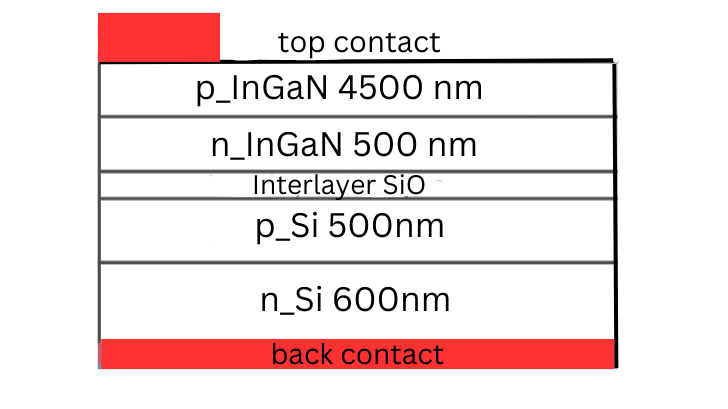
\includegraphics[width=0.7\linewidth]{Figure/Struct}
	\caption{Structure of $InGaN/Si$ tandem solar cell.}
	\label{fig:structure}
\end{figure}

\begin{table}[h!]
	\begin{tabular}{@{}lcccc@{}}
		\toprule
		$Parameters$ & $Unites$ & $GaN$ & $InGaN$ & $Si$ \\ \midrule
		&  &  &  &  \\
		Lattice constant & $A^{o}$ & 5.186 & ... & 5.43 \\
		Electron affinity & $eV$ & 4.1 & 5.44 & 4.05 \\
		Band-gap & $eV$ & 3.42 & 1.9 & 1.2 \\
		Effective mass of electrons ($m_e$) & $m_{0}$ & 0.2 & 0.07 & 0.36 \\
		Heavy effective mass of holes ($m_{hh}$) & $m_{0}$ & 1.4 & 0.7 & 0.81 \\
		Light effective mass of holes ($m_{lh}$) & $m_{0}$ & 0.3 & ... & 0.16 \\
		
		\begin{tabular}[c]{@{}l@{}}Density of states in 
	    \\ the conduction band ($N_c$)
	    \end{tabular} & $cm^{-3}$ & $2.3\times10^{18}$ & ... & $3.2\times10^{19}$ \\
		\begin{tabular}[c]{@{}l@{}}Density of states in \\ the valence band ($N_v$)\end{tabular} & $cm^{-3}$ & $4.6\times10^{19}$ & ... & $1.8\times10^{19}$ \\
		
		Doping concentration of $p$ ($N_A$) & ... & $5\times 10^{17}$ & ... & $6\times 10^{17}$ \\
		Doping concentration of $n$ ($N_D$) & ... &  $5\times 10^{17} $ & ... & $6\times 10^{17} $ \\
		
		Mobility of electrons ($\mu_{e}$) & $cm^{2}/( V.s)$ & 1000 & 300 & 1400 \\
		Mobility of holes ($\mu_{h}$) & $cm^{2}/( V.s)$ & 350 & 50 & 450 \\
		Diffusion coefficient of electrons ($D_{e}$) &$cm^{2}$/s & 25 & ... & ... \\
		Diffusion coefficient of holes ($D_{h}$) & $cm^{2}$/s & 9 & ... & ... \\
		Thermal velocity of electrons ($v_{e}$) & $m/s$ & $2.6\times 10^{5}$ & ... &  \\
		Thermal velocity of holes ($v_{h}$) & $m/s$ & $9.4\times 10^{4}$ & ... & ... \\
		Static relative dielectric constant ($\epsilon_{0}$) & ... & 8.9 & 11.7 & 11.9 \\
		\begin{tabular}[c]{@{}l@{}}High-frequency relative \\ dielectric constant ($\epsilon_{\infty}$)\end{tabular} & ... & 5.35 & ... & ... \\
		\begin{tabular}[c]{@{}l@{}}Surface recombination velocity \\ of minority Electrons  ($S_{n}$)\end{tabular} & $cm/s$ & ... & $1\times 10^{6}$ & $1\times 10^{6}$ \\
		\begin{tabular}[c]{@{}l@{}}Surface recombination velocity \\ of minority holes  ($Sp$)\end{tabular} & $cm/s$ & ... & $1\times 10^{6}$ & $1\times 10^{6}$ \\
		
		Auger recombination for electrons ($R_{A}$) & $cm^{6}s^{−1}$ & ... & $1.5 \times10^{-30}$ & ... \\
		Auger recombination for holes ($R_{A}$) & $cm^{6}s^{−1}$ & ... & $1.5 \times10^{-30}$ & ... \\
					
		Lifetime of minority electrons  ($\tau_{n}$) & $ns$ & ... & 1 & $10^{3}$ \\
		Lifetime of minority holes ($\tau_{p}$) & $ns$ & ... & 1 & $10^{3}$ \\
		Shockley-Read-Hall lifetime ($\tau_{SRH}$) & $ns$ & ... & $1\times 10^{-5}$ & $5\times 10^{-6}$ \\ \bottomrule
	\end{tabular}
	\caption{Parameters used in the electrical simulation. The values for high quality $Si$ are taken from standard references except for
		$\tau_{SRH}$, which is a generic value [Ref.5]. The effective masses are density of state effective masses. Values for high quality $InGaN$ are taken from the literature except for $\tau_{SRH}$ and $B$, which are generic values see [Ref.5]. Values for low quality material are obtained as described in the text.}
	\label{tab:parametres}
\end{table}

\section{Resultat and Discution} \label{sec:R_D}
The energy band diagram under the equilibrium condition of the band alignment of $InGaN$ and $Si$ is illustrated in Fig.\ref{fig:ingansi} can be exploited for the fabrication studied structure of tandem $InGaN/Si$ heterojunctions solar cells that may have power conversion efficiency. To understand of these heterojunctions, a band diagram as shown $ \xi_{1}$ and $ \xi_{2}$ are the electron affinities for both $InGaN$ and $Si$. Therefore, the conduction band of $InGaN$ is below the conduction band of $Si$ and the valence band of $InGaN$ lies below the valence band of $Si$, leading to the formation of a type II heterojunction. The simulation starts from the nominal layer thickness and refractive index calculated using $Wien2k$, and we process this optimization in two stages: Visual simulation to obtain approximate total thicknesses for each link, and then device optimization. Using the $TMM$ simulation to calculate the photogenerated current in each layer, we get an estimate of the total thickness of each material we will need to achieve current matching, from a purely optical point of view the bottom cell $Si$ should be thick to maximize absorption, which of course is not the case for the device. Once we have good values for the layer thicknesses, we use full electrical simulation to determine the n and p thicknesses to calculate the optimal possible efficiency of the tandem solar cell device. Fig.\ref{fig:absref} shows the absorption in each layer using the optimized thicknesses. Now that the layer thickness is optimized from an optical point of view, we want to design the device. Once we have good initial values for the total layer thicknesses, we use full electrical simulation to determine the $n$ and $p$ type layer thicknesses to calculate a maximum possible efficiency. Fig.\ref{fig:iv} shows the calculated voltage-current curves for the best thikness of an $In_{0.54}Ga_{0.46}N/Si$ tandem cell device. The IV curve looks reasonably good.

Fig.\ref{fig:nk} shows us the $n$ and $k$ data for the materials used in this tandem solar cell modeling.
\begin{figure}[h!]
	\centering
	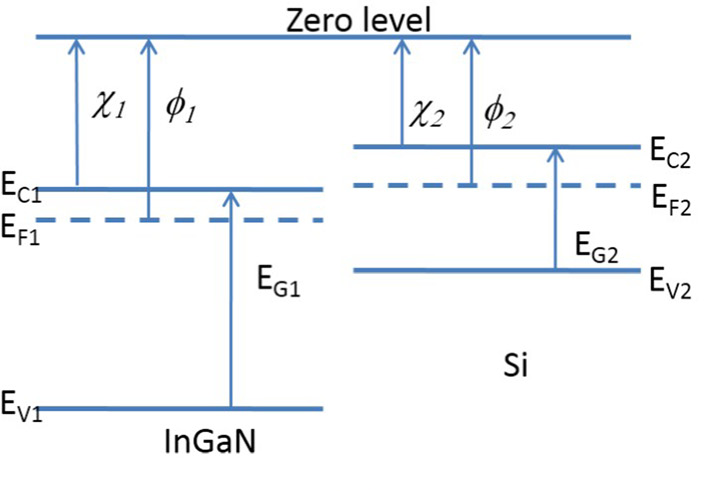
\includegraphics[width=0.7\linewidth, height=0.3\textheight]{Figure/Band}
	\caption{Schematic band diagrams of $InGaN$ and $Si$ before in contact.}
	\label{fig:ingansi}
\end{figure}
\begin{figure}[h!]
	\centering
	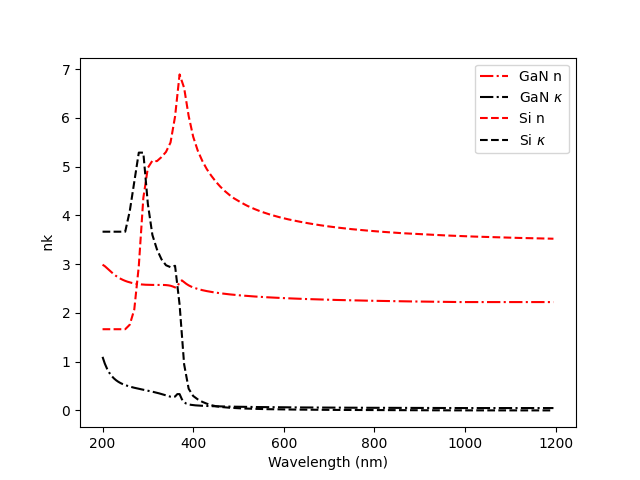
\includegraphics[width=0.7\linewidth, height=0.3\textheight]{Figure/nk}
	\caption{Optical constants of $GaN, InGaN$ and $Si$.}
	\label{fig:nk}
\end{figure}

\begin{figure}[h!]
	\centering
	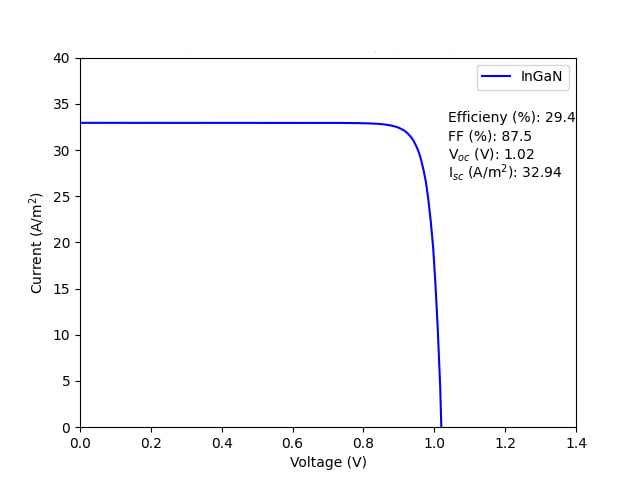
\includegraphics[width=0.45\linewidth,
	height=0.25\textheight]{Figure/IV_InGaN}
	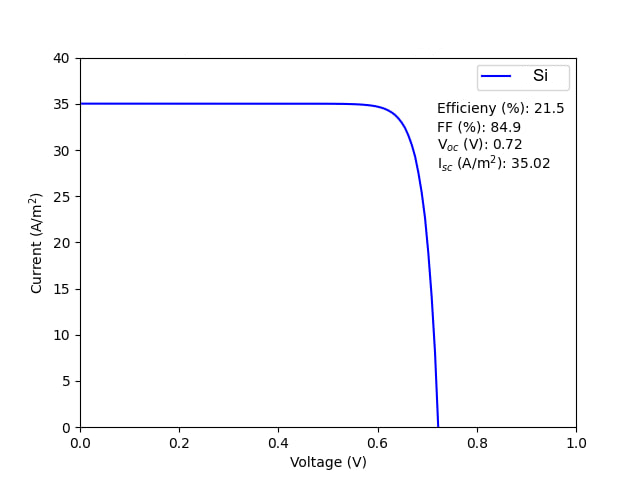
\includegraphics[width=0.45\linewidth, height=0.25\textheight]{Figure/IV_Si}
	\caption{I-V Characteristics of $In_{0.54}Ga_{0.46}N$ and $Si$ Single solar cells.}
	\label{fig:iv}
\end{figure}

\begin{figure}[h!]
	\centering
	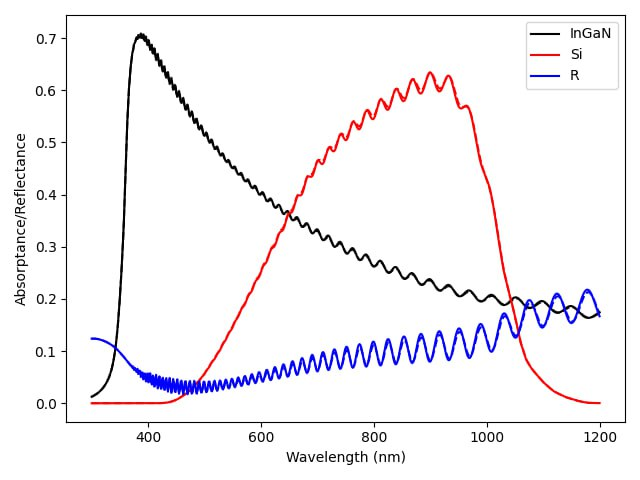
\includegraphics[width=0.45\linewidth, height=0.25\textheight]{Figure/Abs_Ref}
	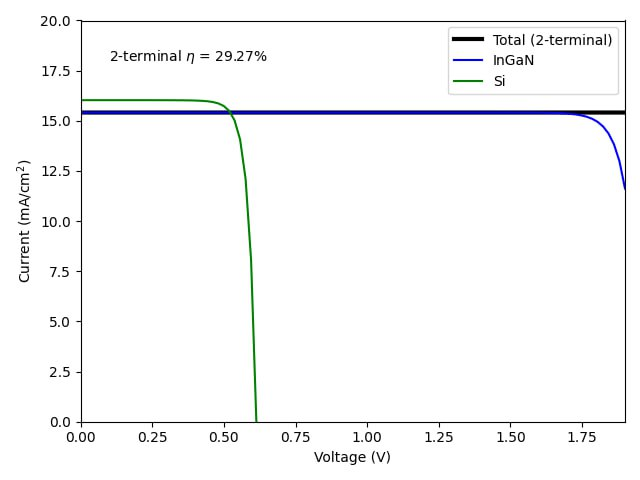
\includegraphics[width=0.45\linewidth, height=0.25\textheight]{Figure/IV}
	\caption{absorption and I-V Characteristics of $In_{0.54}Ga_{0.46}N/Si$ tandem solar cells.}
	\label{fig:abs_iv}
\end{figure}

\begin{table}[h!]
	\begin{tabular}{@{}lcccc@{}}
		\toprule
		& \multicolumn{1}{l}{$J_{sc} (mA/cm^{2})$} & \multicolumn{1}{l}{$V_{oc}$(V)} & \multicolumn{1}{l}{FF (\%)} & 
	    \multicolumn{1}{l}{Efficiency (\%)} \\ \midrule
		$In_{054}Ga_{0.46}N$ & 32.94 & 1.02 & 87.5 & 29.02 \\
		$Si$ & 35.02 & 0.72 & 84.9 & 21.5 \\
		$In_{054}Ga_{0.46}N/Si$ & 34.01 & 1.62 & 91.55 & 30.31\cite{bib14}, 35.2\cite{bib15}, 36.5\cite{bib16}, 37.23\cite{bib17}. 
		 \\ \bottomrule
	\end{tabular}
	\caption{Photovoltaic parameters of the top $InGaN$, bottom $Si$, and tandem $In_{054}Ga_{0.46}N/Si$ cells.}
	\label{tab:result}
\end{table}

From the above table \pageref{tab:result}, it can be said that the $InGaN/Si$ tandem solar cell device gives the best efficiency theoretically, it has not yet been proven due to the intrinsic defects of the cell caused by the high indium content. In this work based on simulation results supported by the electrical and optical characteristics of the device. We found that the addition of 54\% indium to gallium nitride is promising for use in an $InGaN/Si$ solar cell where the top $InGaN$ cell is matched with the bottom $Si$ cell. the solar cell can also be enhanced by optimizing not only the doping and thickness of each solar cell layer, but also by adding indium content as well. 

The improvement in efficiency achieved by adding an $InGaN$ junction to $Si$.  However, for a tandem cell, 1.2 eV is no longer the optimal band-gap for the bottom junction.

\section{Conclusion} \label{sec:Con}

Using Solcore, we theoretically investigated the potential power conversion efficiencies that can be achieved by a tandem $InGaN/Si$ solar cell. There are several limitations such as thickness, band gap, and lattice constant mismatch that need to be considered. Computational models based on $DFT$ theory and the $K.P$ method can provide can provide insight into solar PV cells. Behavioral calculations can be performed, through experimental and theoretical parameters such as index coefficient, band gaps and thicknesses. These formulations are able to model the optical and electrical properties of tandem solar cells. We found that the optimal band gap and top layer thickness of $InGaN$ were \textbf{1.8 eV} and \textbf{600 nm}, respectively, and achieved an optimal conversion efficiency of 30\%, which is higher than that of a single-junction $Si$ solar cell. The obtained results show that an indium content of 54\% is optimal for the tandem $InGaN/Si$ solar cell where the top $InGaN$ cell matches the bottom $Si$ cell. The optimal indium content in the $InGaN/Si$ solar cell is very important in order to optimize the overall performance of the solar cell; open circuit voltage, short circuit current density, fill factor and quantum efficiency. Stacking defects are minimized by introducing an $SiO_{2}$ inter-layer and the current density between the two junctions is matched by choosing an appropriate indium content.

\bibliographystyle{elsarticle-num} 
\bibliography{Ref_Doh.bib}

%% else use the following coding to input the bibitems directly in the
%% TeX file.

%%%%%%%%%%%%\begin{thebibliography}{00}

%% \bibitem{label}
%% Text of bibliographic item

%%%%%%%%%%%%%%%\bibitem{}

%%%%%%%%%%%%%%\end{thebibliography}
\end{document}
%\endinput
